\chapter{Theory}
\label{ch:Theory}

In this section we will discuss the theoretical background the project of this report is based on. As noted in \href{ssec:Objective}{the introduction}, the project aims at developing a proof-of-concept implementation of a Citizen Science accessible Liquid Democracy game. As such, it needs to be grounded in a thorough understanding of both the concept of \href{ssec:Theory_CS}{Citizen Science} and \href{ssec:Theory_LD}{Liquid Democracy}. Additionally it needs to identify and address the problems and issues raised in relation to these concepts. 

In order to address these issues, a discussion of their context is indispensable. In recognition of this, the structure of this section is as follows:
After introducing the basic terms and the context they stem from (in \ref{ssec:Background_CS} and \ref{ssec:Background_LD} respectively), issues and open questions are addressed for both concepts separately (in \ref{ssec:Issues_CS} and \ref{ssec:Issues_LD} respectively). 

Subsequently to a discussion on the background of the respective concept, we will \href{ssec:Integration_CSLD}{discuss synergies and challenges} of integrating these perspectives. Based on this integrative perspective and the aspects discussed at the beginning of this section, we will \href{ssec:Criteria}{derive a number of criteria} a Liquid Democracy game grounded in Citizen Science needs to exhibit, in order to \href{sec:Approach}{develop} a theory-grounded approach to the project's objective.
% Clara
\section{CS}
\label{sec:Theory_CS}
\subsection{Background / Context Citizen Science}
\label{ssec:Background_CS}
Steven is doing that shit. Grundidee CS. Wieso ist die Project Idee geil usw.
\subsection{Issues and Open Questions in Citizen Science}
\label{ssec:Issues_CS}


\section{Liquid Democracy}
\label{sec:Liquid_Democracy}

As there are many forms of political government, it is democracy that spread around the globe over the last hundred years (see \autoref{fig:democracy-trend}). \textit{“As of the end of 2016, 97 out of 167 countries (58\,\%) [\ldots] were democracies [\ldots]”} \parencite{Desilver2017}. According to the observations in \autoref{fig:democracy-trend}) it could be argued that democracy is a very successful and thus modern system, since democracy has no major competitor. Nevertheless, it is not within the scope of this project to asses these systems. Yet, democracy entails various advantages compared to other political systems. For one it entitles its citizens to participate to some extent towards the political process. Additionally, it allows its people to shape the system’s frame. Consequently, democracy comes in many forms. In this project we focus on liquid democracy, a form of democracy that is also known as delegative democracy.


\begin{figure}[H]

	\centering \begin{tikzpicture}
	\node[anchor=south west,inner sep=0] (image) at (0,0,0) {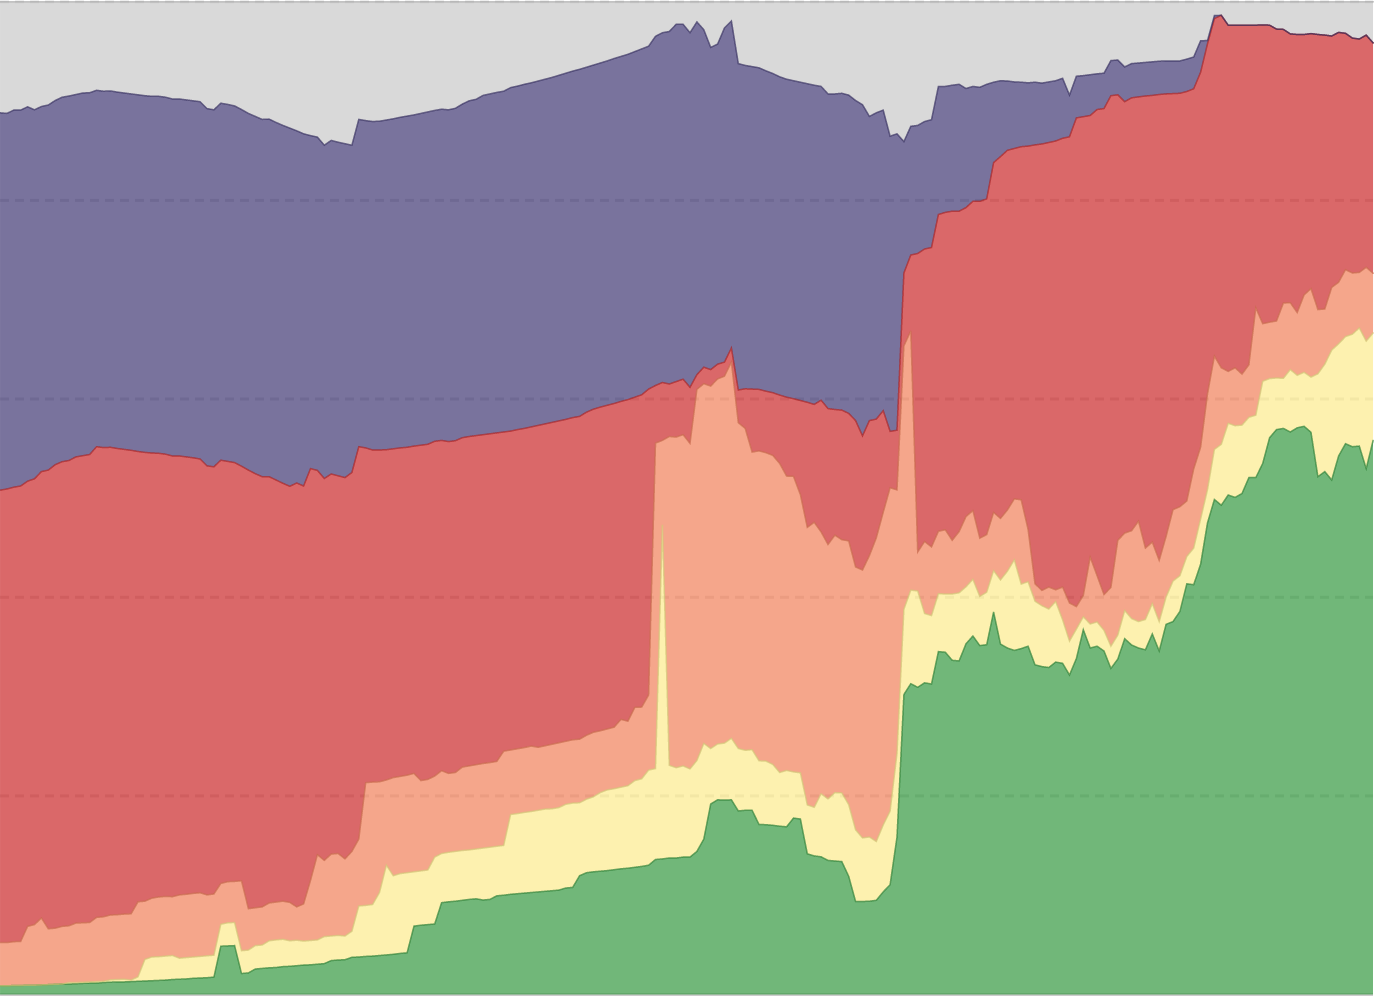
\includegraphics[width=8cm]{democracy-trend.png}};
	\begin{scope}[x={(image.south east)},y={(image.north west)}]
% 	% next four lines will help you to locate the point needed by forming a grid. comment these four lines in the final picture.↓
% 		\draw[help lines,xstep=.1,ystep=.1] (0,0) grid (1,1);
% 		\draw[help lines,xstep=.05,ystep=.05] (0,0) grid (1,1);
% 		\foreach \x in {0,1,...,9} { \node [anchor=north] at (\x/10,0) {0.\x}; }
% 		\foreach \y in {0,1,...,9} { \node [anchor=east] at (0,\y/10) {0.\y};}
% 	% upto here↑
    
	\libertineLF
	\draw (-0.05,0.0) node {\small{0\,\%}};
    \draw (-0.06,0.2) node {\small{20\,\%}};
    \draw (-0.06,0.4) node {\small{40\,\%}};
    \draw (-0.06,0.6) node {\small{60\,\%}};
    \draw (-0.06,0.8) node {\small{80\,\%}};
    \draw (-0.07,1.0) node {\small{100\,\%}};
   	\libertineOsF
    \draw (0.0,-0.06) node {1816};
    \draw (0.17,-0.06) node {1850};
    \draw (0.425,-0.06) node {1900};
    \draw (0.67,-0.06) node {1950};
    \draw (0.93,-0.06) node {2000};
    
	\draw[-latex] (0.99,0.25) -- +(0.5cm,0cm)node[anchor=west] {\scriptsize{Democracy}};
    \draw[-latex] (0.99,0.6) -- +(0.5cm,0cm)node[anchor=west] {\scriptsize{Open Anocracy}};
    \draw[-latex] (0.99,0.695) -- +(0.5cm,0cm)node[anchor=west] {\scriptsize{Closed Anocracy}};
    \draw[-latex] (0.99,0.85) -- +(0.5cm,0cm)node[anchor=west] {\scriptsize{Autocracy}};
    \draw[-latex] (0.99,0.96) -- +(0.5cm,-0.28cm)node[anchor=west] {\scriptsize{Colony}};
    \draw[-latex] (0.99,0.98) -- +(0.5cm,0cm)node[anchor=west] {\scriptsize{Transition/No data}};

	
	\end{scope}
	\end{tikzpicture}
	\caption[World population by political regime they live in]{World population by political regime they live in \parencite[see][]{Roser2018}.}
	\label{fig:democracy-trend}

\end{figure}


\subsection{Background}
\label{ssec:Background_LD}

\acrfull{LD} 

\subsection{Issues and Open Questions in Liquid Democracy}
\label{ssec:Issues_LD}
\section{An Integrative Perspective for Citizen Science in Liquid Democracy}
\label{sec:Integration_CSLD}

\subsection{Data Accessibility and Anonymity}
\label{ssec:Integration_AccessibilityAnonymity}
Arguably the most challenging aspect of a CS-based LD platform, is the tension between data accessibility and anonymity. As stressed \todo{actually stress it!} in \ref{ssec:Issues_LD}, vote anonymity is a crucial aspect of democratic voting systems. On the other hand, a lack of transparency and data accessibility \todo[inline]{reduces the Citizen Scientist} to a data provider, devoiding a system of its participatory nature and transforming it into a mere crowd-sourcing platform (from a CS perspective). In order to allowing Citizens to pose (and investigate) research questions based on real-world data within their context of interest and expertise, as well as for delegators to evaluate whether their values are represented appropriately by delegants, data accessibility / transparency (at least to some degree) is imperative.

Although at first glance transparency and anonymity might seems like a null-sum-game where increased data accessibility constitute a violation of a users privacy, a number of strategies do exists that tackle these problems.

\subsubsection{Decoupling User Accounts from Personal Identity}

The most obvious strategy might be to decouple the user account from the personal identity of a user. When done consecuently, with proper protection of data (and the personal identity of the user is used solely to validate the vote connected to the account, or even just the existence of the account), all data of the user can be transparent by everyone, and no restrictions on the data accessiblity needs to be enforced. While this is the optimal solution from the perspective of the Citizen Scientist, and the delegator that can (in theory) perfectly evaluate whether her political power was used as intended, this approach is not without danger.

First, and most obviously, this approach is very problematic when a breach of the separation of the user and personal identity of the user occurs. Perfect safety does not exist, and many cases where sensitive (and this would be highly sensitive) information was exposed do exist (citation needed). More subtly however, with perfect accessibility of user data, with more and more detailed data, increasingly detailed profiles can be constructed, which are more and more likely to be bound to a person by tying their democratic persona to their personal identity (citation needed). While this might be somewhat harder for 'non-public' persons, for people active in the public sphere by their personal identities (e.g. politicians), this link would be easy to establish. One thoughtless given detail might be enough to link the entirety of the user persona to the human behind their account, making transparent in its entirety all activity and views every uttered on the platform. 

Most problematic about this issue from a participatory democratic perspective is the mechanics that more involvement leads to a higher probability of (someone sufficiently clever) the user persona being linked to the person behind this, thus rather discouraging than encouraging engagement in the participatory processes.

\subsubsection{Aggregating User Data}

Another, rather conservative solution for this issue would be to anonymize the user data by aggregating voting behaviour by demographic aspects of users. A scientist would thus get access to the distribution of voting patterns, vote delegation patterns or involvement in issues by certain demographics. Though preserving the anonymity and privacy integrity of the person behind a user, it has two shortcomings. First, this employs a conservative empiric perspective (since science by demography is out and attitude and behaviour, as well as cognitive patterns are en vogue (citation needed)). Second, this enables the interested scientist only to ask one type of question. The form of the research question is thus already pre-determined by the designers of the platform, and the demographic categories users provide. While this doesn't hinder Citizen Scientists to design and perform studies on the data, this doesn't realize the high participatory level of involvement in the research process that we would strive for in this project.

An aspect not addressed by this perspective is how much information a delegator would receive about the delegant (and the delegants it re-delegates the vote to). Since the usage of the single vote of the delegant is of interest, an aggregated perspective does not answer how well he could ensure his values are respected. With absolute transparency of the behaviour of the delegant to the delegator, a malign and smart (group of) delegators could derive information that would validate this paradigm.

\subsubsection{Deflecting Responsibility}

An easy, yet cowardish, third option for dealing with this problem would be to shift the responsibility for this from the platform's designers or operators to the users. Users could decide how much information they want to make available to other users / scientists and their delegators. While this has the chance to solve the problem and pay users the respect of being mature enough to decide this, this might lead to transparency pressure that every user that wants to accumulate political power needs to justify himself. Maybe deciding to pay this price is what can be expected from a politician, but this decision should not be engrained in the architecture of the platform. How easy such a setup would be for a scientist who has to deal with (potentially a lot of) partial information needs to be evaluated.

\subsubsection{Selective Aggregation}

A further, much more involved option would be to 'hide' unaggregated information for inquiring scientists, and to allow only information of a certain level of aggregation. Though similar to the second option posed above, this is quite a different approach to the problem at hand, since this approach explicitly opposes restricting research questions to a set / style of pre-formed research questions. The idea behind this approach is to allow all \textit{kind} of data inquiries, as long as certain criteria are met. These criteria are thought to ensure the anonymity of the user identity against inquiring entities, and would be the main design issue of this concept. As an example, criteria could be quantitative, only allowing access to data with a given amount of entities. This could be realized e.g. through a data query language with a filter instance, only allowing responses on data instances of a given size (in the style of 'how many people that voted like this in elections of this context voted like that / delegated votes' with a negative response when there are only a handful of instances and a valid answer when there are a substantial number of instances). Establishing these criteria would probably result in a lot of (hard) work, but might well be worth it. Whether research would be possible with the partial answers this approach generates, is a different question altogether. 
This approach further doesn't give an answer to transparency of vote delegation for individual political subjects raised above.

%\subsection{Theorien aus Liquid Feedback}
\section{Criteria for a CS based LD Platform}
\label{sec:Criteria}